%% Direttive TeXworks:
% !TeX root = ./presentazione.tex
% !TEX encoding = UTF-8 Unicode
% !TEX program = arara
% !TEX TS-program = arara
% !TeX spellcheck = it-IT

%! arara: clean: { files: [ arara.log, presentazione.aux, presentazione.log, presentazione.nav, presentazione.out, presentazione.snm, presentazione.toc, presentazione.xmpdata, pdfa.xmpi, presentazione.pdf ] }
% arara: clean: { files: [ arara.log, presentazione.log, presentazione.xmpdata, pdfa.xmpi, presentazione.pdf ] }
% arara: pdflatex: { shell: yes, synctex: yes, action: batchmode, options: "-halt-on-error -file-line-error-style" }
% arara: biber
% arara: pdflatex: { shell: yes, synctex: yes, action: batchmode, options: "-halt-on-error -file-line-error-style" }
% arara: pdflatex: { shell: yes, synctex: yes, action: nonstopmode, options: "-halt-on-error -file-line-error-style" }

%%%%%%%%%%%%%%%%%%%%%%%%%%%%%%%%%%%%%%%%%%%%%%%%%%%%%%%%
%% Genera un file report.xmpdata con i dati per PDF/A %%
\begin{filecontents*}{\jobname.xmpdata}
\Title{RxJS: Reactive Extensions For JavaScript}
\Author{Niccolò Maltoni}
\Copyright{Copyright \copyright 2018, Niccolò Maltoni}
\CopyrightURL{http://creativecommons.org/licenses/by-nc-sa/3.0/it/}
\Keywords{RxJS\sep ReactiveX\sep JavaScript\sep JS}
\end{filecontents*}
%%%%%%%%%%%%%%%%%%%%%%%%%%%%%%%%%%%%%%%%%%%%%%%%%%%%%%%%

\documentclass{beamer}

%%%%%%%%%%%%%%%%%%%%%%%%%%%%%%%%%%%%%%%%%%%%%%%%%%%%%%%%%%%%
%% Imposto la codifica del sorgente e del testo in uscita %%
\usepackage[T1]{fontenc}        % serve per impostare la codifica di output del font
\usepackage{textcomp}           % serve per fornire supporto ai Text Companion fonts
 \usepackage[utf8]{inputenc}     % serve per impostare la codifica di input del font
\usepackage[
    english,            % utilizza l'inglese come lingua secondaria
    italian             % utilizza l'italiano come lingua primaria
]{babel}                        % serve per scrivere Indice, Capitolo, etc in Italiano
\usepackage{lmodern}            % carica una variante Latin Modern prodotto dal GUST
%%%%%%%%%%%%%%%%%%%%%%%%%%%%%%%%%%%%%%%%%%%%%%%%%%%%%%%%%%%%

\usepackage{graphicx}           % serve per includere immagini e grafici

\usepackage{listings}
\usepackage{minted}

\usepackage[%
    strict,             % rende tutti gli warning degli errori
    autostyle,          % imposta lo stile in base al linguaggio specificato in babel
    english=american,   % imposta lo stile per l'inglese
    italian=guillemets  % imposta lo stile per l'italiano
]{csquotes}                     % serve a impostare lo stile delle virgolette

\usepackage[%
    maxcitenames=2,     % massimo numero di nomi nelle citazioni
    mincitenames=2,     % minimo numero di nomi nelle citazioni
    maxbibnames=99,     % massimo numero di nomi nella blibliografia
    minbibnames=99,     % minimo numero di nomi nella blibliografia
    style=numeric,
    giveninits=true,
    backend=biber       % specifica il backend per la bibliografia
]{biblatex}                     % si interfaccia con bibtex e biber per la bibliografia
\addbibresource{biblio.bib}

\setcounter{secnumdepth}{2}     % Numera fino alla sottosezione nel corpo del testo
\setcounter{tocdepth}{3}        % Numera fino alla sotto-sottosezione nell'indice

\graphicspath{{img/}}

\usepackage[%
    depth=3,            % equivale a bookmarksdepth di hyperref
    open=false,         % equivale a bookmarksopen di hyperref
    numbered=true       % equivale a bookmarksnumbered di hyperref
]{bookmark}                     % Gestisce i segnalibri meglio di hyperref
\usepackage{hyperref}           % Gestisce tutte le cose ipertestuali del pdf
\hypersetup{%
    pdfpagemode={UseNone},
    hidelinks,          % nasconde i collegamenti (non vengono quadrettati)
    hypertexnames=false,
    linktoc=all,        % inserisce i link nell'indice
    plainpages=false,
    breaklinks,
    pdfstartview={Fit},
    unicode=true,       % only Latin characters in Acrobat's bookmarks
    pdftoolbar=false,   % show Acrobat's toolbar?
    pdfmenubar=false,   % show Acrobat's menu?
    plainpages=false
}
\usepackage[pdf15,a-1b]{pdfx}

%%%%%%%%%%%%%%%%%%%%%%%%%%%
%% Impostazione del tema %%
\usetheme{Boadilla}             % serve per scegliere il layout generale dei frame
\definecolor{darkrxpurple}{RGB}{87,43,139}
\definecolor{rxpurple}{RGB}{216,26,96}
\colorlet{primarygrey}{gray!30!white}
\colorlet{secondarygrey}{gray!15!white}
\colorlet{terziarygrey}{gray!10!white}
\colorlet{greyrxpurple}{rxpurple!75!secondarygrey}
\definecolor{lighrxpurple}{RGB}{236,12,144}
\colorlet{greylightrxpurple}{lighrxpurple!25!terziarygrey}
\usecolortheme{beaver}          % Per il colore va comunque bene questo
% \usecolortheme[named=rxpurple]{structure}
\setbeamerfont{block title}{size=\normalsize}
\setbeamerfont{block body}{size=\small}
\setbeamertemplate{navigation symbols}{}  % nasconde i controlli di presentazione
\setbeamercolor{palette primary}{fg=darkrxpurple, bg=greylightrxpurple}
\setbeamercolor{palette secondary}{fg=white, bg=lighrxpurple}
\setbeamercolor{palette tertiary}{fg=white, bg=darkrxpurple}
% \setbeamercolor{title}{fg=white}
% \setbeamercolor{subtitle}{fg=white}
\setbeamercolor{title}{fg=white, bg=darkrxpurple}
\setbeamercolor{subtitle}{fg=white, bg=darkrxpurple}
\setbeamercolor{frametitle}{fg=rxpurple}
\setbeamercolor{framesubtitle}{fg=rxpurple}
\setbeamercolor{block title}{fg=darkrxpurple}

\renewcommand{\thefootnote}{\arabic{footnote}}
%%%%%%%%%%%%%%%%%%%%%%%%%%%

%%%%%%%%%%%%%%%%%%%%%%%%%%%%%%%%%%%%%%%%%%%%%%%%%%%%%%%%%%%%%%%%%%%%
%% Definisco un nuovo comando per enfatizzare il testo in inglese %%
\newcommand{\engEmph}[1] {\emph{\foreignlanguage{english}#1}}
%%%%%%%%%%%%%%%%%%%%%%%%%%%%%%%%%%%%%%%%%%%%%%%%%%%%%%%%%%%%%%%%%%%%

%%%%%%%%%%%%%%%%%%%%%%%%%%%%%%%%%%%%%%%%%%%%%%%%%%%%%%%%%%
%% Permette di inserire l'outline prima di ogni sezione %%
\AtBeginSection[]{%
    \begin{frame}<beamer>
        \frametitle{Outline}
        \tableofcontents[currentsection]
    \end{frame}
}
%%%%%%%%%%%%%%%%%%%%%%%%%%%%%%%%%%%%%%%%%%%%%%%%%%%%%%%%%%

%%%%%%%%%%%%%%%%%%%%%%%%%%%%%%%%%%%%%%%%%%%%%%%%%%%%%%%%%%%%%%%
%% Permette di inserire automaticamente titolo e sottotitolo %%
% \addtobeamertemplate{frametitle}{
%    \let\insertframetitle\insertsectionhead}{}
% \addtobeamertemplate{frametitle}{
%    \let\insertframesubtitle\insertsubsectionhead}{}

% \makeatletter
%   \CheckCommand*\beamer@checkframetitle{\@ifnextchar\bgroup\beamer@inlineframetitle{}}
%   \renewcommand*\beamer@checkframetitle{\global\let\beamer@frametitle\relax\@ifnextchar\bgroup\beamer@inlineframetitle{}}
% \makeatother
%%%%%%%%%%%%%%%%%%%%%%%%%%%%%%%%%%%%%%%%%%%%%%%%%%%%%%%%%%%%%%%

\title[RxJS]{ReactiveX RxJS}
\subtitle{Reactive Extensions For JavaScript}
\author[Niccolò~Maltoni]{\large{Niccolò~Maltoni}\\{\small\texttt{niccolo.maltoni@studio.unibo.it}}}
\date[30 maggio 2018]{}
\institute[0000840825]{
\includegraphics[scale=.4]{Rx_Logo}}

\begin{document}
    \begin{frame}[c]
        \titlepage
    \end{frame}

    \section{Introduzione}\label{sec:intro}
        \subsection{Programmazione reattiva}\label{subsec:react}
        \begin{frame}{\insertsectionhead}
            \begin{block}{\insertsubsectionhead}
                \smallskip
                \begin{quote}
                    \foreignlanguage{english}
                    `` It is convenient to distinguish roughly between three kinds of computer programs.
                    Transformational programs compute results from a given set of inputs;
                    typical examples are compilers or numerical computation programs.
                    Interactive programs interact at their own speed with users or with other programs;
                    from a user point of view, a time-sharing system is interactive.
                    \textbf{Reactive programs also maintain a continuous interaction with their environment, but at a speed which is determined by the environment, not the program itself}.
                    Interactive programs work at their own pace and mostly deal with communication, while reactive programs only work in response to external demands and mostly deal with accurate interrupt handling. ''
                \end{quote}
                \rightline{Gérard~Berry,~1989~\cite{berry:inria-00075494}}
            \end{block}
        \end{frame}

        \subsection{Reactive Manifesto}\label{subsec:manifest}
        \begin{frame}{\insertsectionhead}
            \begin{block}{\insertsubsectionhead~\cite{citeulike:13845446}}
                \begin{itemize}
                    \item
                        Prima versione presentata nel 2013.
                    \item
                        Principi base:
                        \begin{itemize}
                            \item responsività;
                            \item resilienza;
                            \item scalabilità;
                            \item \engEmph{event-driven}.
                        \end{itemize}
                    \item
                        La versione attuale (2.0) è stata presentata l'anno successivo~\footnotemark.
                        \begin{itemize}
                            \item da scalabilità a \textbf{elasticità};
                            \item da \engEmph{event-driven} a \textbf{\engEmph{message-driven}}.
                        \end{itemize}
                \end{itemize}
            \end{block}
            \footnotetext{\url{https://www.lightbend.com/blog/reactive-manifesto-20}}
        \end{frame}

        \begin{frame}[c]{\insertsectionhead}{\insertsubsectionhead}
        % \begin{block}{\vspace*{-3ex}}
            \begin{figure}[htbp]
                \centering
                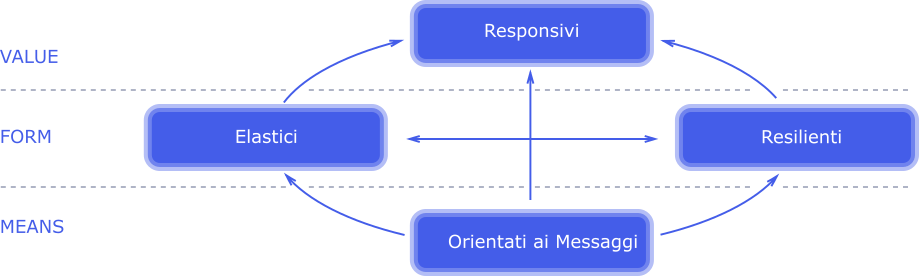
\includegraphics[width=\linewidth]{reactive-traits-it}
                \caption{Rappresentazione dei principi base del \engEmph{Reactive Manifesto}}
                \label{fig:manifest}
            \end{figure}
        % \end{block}
        \end{frame}

        \begin{frame}[c]{\insertsectionhead}{\insertsubsectionhead}
            \begin{columns}
                \begin{column}{.47\textwidth}
                    \centering
                    \subsubsection{Responsività}\label{subsub:responsive}
                    \begin{block}{\insertsubsubsectionhead}
                    \begin{itemize}
                        \item \textbf{tempestività} della risposta
                        \begin{itemize}
                            {
                                \footnotesize
                                \item rapida identificazione dei problemi
                                \item minimizzazione del tempo di risposta
                            }
                        \end{itemize}
                        \item garanzia di \textbf{qualità del servizio} nel tempo
                        \item \textbf{predicibilità} del comportamento
                        \begin{itemize}
                            {
                                \footnotesize
                                \item semplificazione della gestione degli errori
                                \item fiducia degli utenti finali nel sistema
                            }
                        \end{itemize}
                    \end{itemize}
                    \end{block}
                \end{column}
                \begin{column}{.47\textwidth}
                    \centering
                    \subsubsection{Resilienza}\label{subsub:resiliency}
                    \begin{block}{\insertsubsubsectionhead}
                        \begin{itemize}
                            \item
                                il sistema resta \textbf{responsivo anche in caso di guasti}
                            \item
                                garantita tramite:
                                \begin{itemize}
                                {
                                    \footnotesize
                                    \item replica
                                    \item contenimento
                                    \item isolamento
                                    \item delega
                                }
                            \end{itemize}
                        \end{itemize}
                    \end{block}
                \end{column}
            \end{columns}
        \end{frame}
        \begin{frame}[c]{\insertsectionhead}{\insertsubsectionhead}
            \begin{columns}
                \begin{column}{.47\textwidth}
                    \centering
                    \subsubsection{Elasticità}\label{subsub:elasticity}
                    \begin{block}{\insertsubsubsectionhead}
                    \begin{itemize}
                        \item
                            il sistema rimane \textbf{responsivo sotto carichi di lavoro variabili} nel tempo
                        \item
                            \textbf{adattabilità} attraverso incremento o decremento delle risorse allocate al processamento degli input
                            \begin{itemize}
                            {
                                \footnotesize
                                \item no sezioni contese né colli di bottiglia
                                \item distribuibilità
                                \item replica dei componenti
                                \item ripartizione degli input
                            }
                            \end{itemize}
                        \item possibile implementazione predittiva
                    \end{itemize}
                    \end{block}
                \end{column}
                \begin{column}{.47\textwidth}
                    \centering
                    \subsubsection{\engEmph{Message-Driven}}\label{subsub:meddagedriven}
                    \begin{block}{\insertsubsubsectionhead}
                        \begin{itemize}
                            \item
                                \textbf{scambio di messaggi asincrono}
                                \begin{itemize}
                                {
                                    \footnotesize
                                    \item stile di comunicazione non bloccante
                                }
                                \end{itemize}
                            \item
                                basso accoppiamento tra i componenti
                            \item
                                isolamento e trasparenza sul dislocamento
                            \item
                                esprimere i guasti del componente sotto forma di messaggi
                        \end{itemize}
                    \end{block}
                \end{column}
            \end{columns}
        \end{frame}

        \subsection{Reactive Extensions}\label{subsec:rx}
        \begin{frame}{\insertsectionhead}
            \begin{block}{\insertsubsectionhead}
                \begin{itemize}
                    \item
                        Reactive Extensions (o \textbf{ReactiveX}) sono un set di librerie per la maggior parte dei linguaggi e dei framework moderni che permette l'implementazione di programmi in grado di operare su sequenze di dati e input in modo \textit{reattivo} e \textit{asincrono}, indipendentemente dalla natura della sorgente
                    \item
                        ispirate alle \engEmph{Microsoft's Reactive Extensions} per ambiente .NET
                    \item
                        combinazione di:
                        \begin{itemize}
                        {
                            \footnotesize
                            \item pattern Observer
                            \item pattern Iterator
                            \item programmazione funzionale
                        }
                        \end{itemize}
                \end{itemize}
            \end{block}
            \begin{figure}[htbp]
                \centering
                
\includegraphics[scale=.35]{Rx_Logo_Text}
                \label{fig:rx}
            \end{figure}
        \end{frame}

    \section{RxJS: Reactive Extensions Library for JavaScript}\label{sec:rxjs}
        \subsection{Reactive Extensions for JavaScript}\label{subsec:rxjs}
        \begin{frame}[fragile]{\insertsectionhead}

            \begin{block}{\insertsubsectionhead\footnotemark}
                \begin{itemize}
                    \item
                        RxJS è una libreria per la programmazione reattiva pensata per JavaScript.
                    \item
                        semplifica l'implementazione di \engEmph{callback} e chiamate asincrone attraverso il tipo \texttt{Observable} e i suoi costrutti satelliti, come:
                        \begin{itemize}
                            \item \texttt{Observer}
                            \item \texttt{Schedulers}
                            \item \texttt{Subjects}
                            \item operatori come \texttt{map}, \texttt{filter}, \texttt{reduce}, \texttt{every}, ecc ...
                        \end{itemize}
                \end{itemize}
            \end{block}

            \subsubsection{Installazione}\label{subsec:install}
            \begin{block}{\insertsubsubsectionhead}
                \begin{itemize}
                    {
                        \footnotesize
                        \item
                            Via \textbf{\small\url{npm}}:
                            \inputminted[fontsize=\scriptsize]{text}{res/npm_install.sh}
                        \item
                            Via \textbf{\footnotesize CDN}:
                            \inputminted[fontsize=\scriptsize]{text}{res/cdn_install.html}
                    }
                \end{itemize}
            \end{block}

            \footnotetext{\url{http://reactivex.io/rxjs}}
        \end{frame}
        
        \subsection{Costrutti fondamentali}\label{subsec:costrutti}
            \subsubsection{Observable}\label{subsec:observable}
            \begin{frame}{\insertsubsectionhead}
                \begin{block}{\texttt{\insertsubsubsectionhead}}
                    Pippo
                \end{block}
            \end{frame}
    \nocite{*}
    \section{\refname}\label{sec:ref}
    \begin{frame}[t,allowframebreaks]
        \frametitle{\insertsectionhead}
        \printbibliography
    \end{frame}
\end{document}
